\section{Umsetzung}

In diesem Kapitel wird beschrieben, wie die Anforderungen praktisch
umgesetzt wurden. Zunächst wird darauf eingegangen, wie Shapes gezeichnet
werden, danach wie Spray passenden Code für Spray Web generieren kann
und zuguterletzt wie Spray Web Modelle validiert und persistiert.

\subsection{Shapes zeichnen}

Es ist essentiell dass die Basisshapes gezeichnet werden können.
Zudem sollen die Basisshapes die in Kapitel \ref{sec.primitivShapes}
beschrieben sind, auch ineinander verschachtelbar sein.
Da die Shapes auch u.a. Textfelder enthalten können, um z.B. das Shape
zu benennen, ist es nötig dass der Benutzer diese verändern kann auch
innerhalb eines verschachtelten Shapes.
Da die Shapes mit Connections zusammen eine Graphstruktur bilden,
müssen die Shapes über Connections miteinander verbunden werden können.

Es wäre ideal, wenn ein Toolkit existieren würde, welches all diese
Anforderungen erfüllt. Falls ein solches Toolkit nicht existiert,
müsste selbst eines mit den in Kapitel \ref{sec.funcAnforderung}
gestellten Anforderungen gebaut werden.

\paragraph{SVG oder Canvas?} Für diesen kontreten Anwendungsfall ist
SVG die bessere Wahl, siehe dazu Abbildung \ref{fig.svgVsCanvas}.
Ein Hauptgrund\footnote{Vgl. \url{http://dev.opera.com/articles/view/svg-or-canvas-choosing-between-the-two/}} ist u.a. auch, dass weniger Zeilen Code benötigt werden
als bei Canvas (selbst wenn man auf entsprechende Toolkits zurückgreift)
und direkt Vektorgrafiken produziert werden.

\begin{figure}[h!]
  \centering
  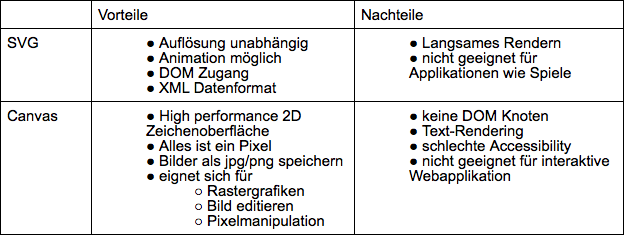
\includegraphics[width=1.0\textwidth]{Figures/Svg_vs_Canvas.png}
  \caption{SVG versus Canvas.}\label{fig.svgVsCanvas}
\end{figure}


\subsubsection{Toolkits}

Folgende Toolkits haben wir auf ihre Tauglichkeit überprüft:

\begin{itemize}
  \item d3.js \\
  Ist ein Toolkit um im Web interaktive Diagramme darzustellen und
  verwendet dabei SVG.
  \item kinetic.js \\
  Ist eine Bibliothek, um eine komfortablere API zu Canvas anzubieten
  und wurde von Simon Schneeberger bereits verwendet.
  \item Raphael.js \\
  Ist ähnlich zu kinetic.js.
  \item LucidCharts \\
  Ist ein Editor ähnlich zu Visio, jedoch im Web mit HTML/CSS/JavaScript,
  setzt auf Canvas.
  \item \dd
  Bietet eine ähnliche API wie das aus der Java-Welt bekannte Draw2d,
  es ist in der Lage Shapes und Connections zu zeichnen.
  Verwendet SVG.
  \item go.js
  Ist ähnlich zu \dd, jedoch nicht Quelloffen.
\end{itemize}

\subsubsection{\dd}

Erst relativ spät haben wir das \dd~Toolkit gefunden.
Es erfüllt quasi alle Anforderungen (siehe Abb. \ref{fig.ddCheck})
und ist damit der Gewinner unter den
durch unsere Recherche untersuchten Toolkits.

\begin{figure}[h!]
  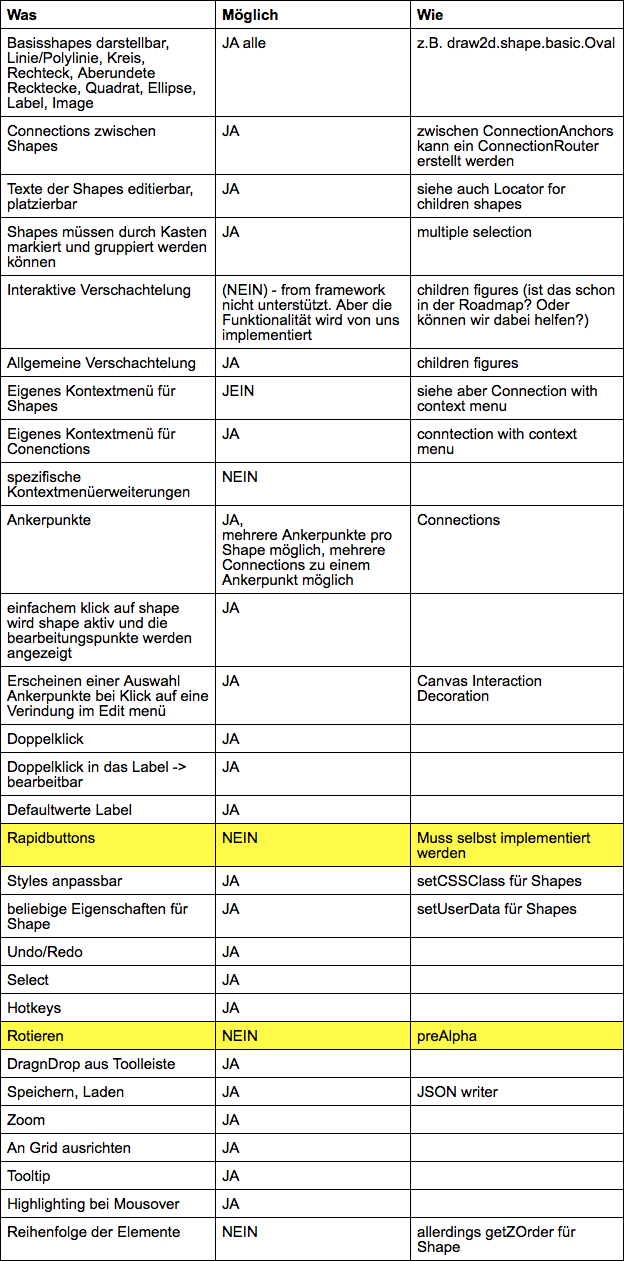
\includegraphics[height=0.9\textheight]{Figures/DD_Anforderungen.png}
  \caption{\dd~Anforderungsüberprüfung.}\label{fig.ddCheck}
\end{figure}

\noindent \dd~wurde von \citep{dd} entwickelt und steht u.a. unter der GNU General
Public Lizenz (GPL) und ist daher auch rein rechtlich geeignet für
das ebenfalls unter einer Open Source Lizenz stehende Spray-Projekt.

\subsubsection{Shape Factory}

Rekursives Zeichnen der Shapes aus einer Definition

\subsubsection{Compartments}


\subsection{Code-Generierung}

Spray Web ist so aufgebaut, dass es von Spray generierten Code annimmt
und verarbeitet. Da Spray intern um andere Generator-Implementierungen
erweiterbar ist, ist es auch möglich, dass ideal für Spray Web
zugeschnittenen Code erzeugt werden kann.

Die Generatoren sind in Xtend geschrieben, dieses ist wiederrum Teil
der Language Workbench
\emph{Xtext}\footnote{Siehe \url{http://www.eclipse.org/Xtext/}}.

\subsubsection{Shape Layout Definitionen}

Es soll JSON-Code aus der Shape Grammatik \citep[gemäß][]{sprayUser}
generiert werden. Der Code befindet sich im Repositorium in
{\tt generators/shape\_dsl/ShapeGenerator.xtend}.
Ziel ist es z.B. aus folgender Spray-Shape-Grammatik:

\begin{verbatim}
shape TransitionShape {
  text {
    position (x=0, y=0)
    size (width=30, height=30)
    id = transitionText
  }
  rectangle {
    position(x=0, y=30)
    size (width=40, height=40)  
  }
}
\end{verbatim}

\noindent Ein solches JSON zu generieren:

\begin{verbatim}
{
  name: "TransitionShape",
  params: {
    size: {witdh: 40, height: 70}
  },
  shapes: [
    {
      name: "Text",
      params: {
        size: {width: 30, height: 30},
        align: {
          horizontal: "left",
          vertical: "top"
        }
      }
    },
    {
      name: "Rectangle",
      params: {
        size: {width: 40, height: 40},
      }
    }
  ]
}
\end{verbatim}

\paragraph{JSON Shape Spezifikation}
Komplexe Shapes können aus primitiven Shapes zusammengesetzt werden.
Es gibt folgende primitive Shapes:

\begin{itemize}
  \item Line
  \item PolyLine
  \item Rectangle
  \item RoundedRectangle
  \item Polygon
  \item Ellipse
  \item Text
  \item Anchor
\end{itemize}

\noindent Diese komplexen Shapes werden in einer Datei {\tt genshape.js} in einer
JSON-Datenstruktur abgelegt. Die Datei enthält eine Variable, worin die
Shapes in einer Liste abgespeichert werden:

\begin{verbatim}
var shapedefs = [
  {...},
  {...},
  ...
]
\end{verbatim}

\noindent Jedes \verb|{...}| Objekt entspricht genau einem komplexen Shape.
Jedes dieser Shapes kann folgende Eigenschaften (JSON Properties) besitzen:

\begin{verbatim}
  name    : "..."
  params  : {...}
  anchors : [...]  (only in the top level!)
  shapes  : [...]
\end{verbatim}

\noindent {\tt name} beschreibt entweder das primitive Shape oder wenn es ganz oben
in der Hierarchie steht den Namen des komplexen Shapes.
In {\tt params} können wieder folgende Attribute vorkommen:

\begin{verbatim}
  position : [{x: Int, y: Int, radius: Int, angle: Int, offset: Float}*]
  size : {width: Int, height: Int}
  stretching : {horizontal, vertical}
  align : {horizontal, vertical}
    horizontal : "left" | "center" | "right"
    vertical :  "top" | "middle" | "center"
  curve : {width: Int, height: Int}
  size-min : {width: Int, height: Int}
  size-max : {width: Int, height: Int}
  proportional : Bool
  layout : {stretching | spacing : Int | margin : Int | invisible}
  points : [{x: Int, y: Int, curveBefore: Int, curveAfter: Int}*]
\end{verbatim}

\noindent Nur in der obesteren Ebene der Hierarchie können Anker {\tt anchors} definiert werden,
diese betreffen also nur das gesamte komplexe Shape (Anker können also
nicht verschachtelt werden). Es gibt diese Formen von Ankern:

\begin{verbatim}
  {type: "center"}
  {type: "corners"}
  {type: "relative", x: Int, y: Int}
  {type: "fixpoints", x: Int, y: Int}
\end{verbatim}

\noindent Mit der {\tt shapes} Property kann die Verschachtelung des Shapes beschrieben
werden, es darf also die gesamte Shape-Definition hier nochmals (also
rekursiv) vorkommen.

Folgende Parameter dürfen nur in der obersten Ebene der Hierarchie innerhalb
der {\tt params}-Liste vorkommen:

\begin{verbatim}
  minWidth: Int
  minHeight: Int
  maxWidth: Int
  maxHeight: Int
  stretchH: Bool
  stretchV: Bool
  proportional: Bool
\end{verbatim}

\noindent Zudem wird immer für das insgesamte komplexe Shape eine Boundingbox berechnet,
d.h. es existiert in der obestern Ebene immer ein {\tt size}-Objekt innerhalb
der {\tt params}.

\paragraph{Compartments} sind spezielle Shapes, die andere Shapes wiederrum
zur Laufzeit aufnehmen können. Es können nur Rectangle und Ellipse als
Compartment markiert werden, d.h. sie enthalten innerhalb ihres {\tt params}
Property folgendes Attribut:

\begin{verbatim}
  compartment: {
    locationId: String,
    layout: fixed|vertical|horizontal|fit,
    spacing: Int,
    margin: Int,
    insisible: Bool,
    stretchH: Bool,
    stretchV: Bool
  }
\end{verbatim}

\paragraph{Connections} sind ebenfalls ein Spezialfall von Shape,
welche sich jedoch explizit von den „normalen“ Shapes unterscheiden,
denn sie können nur folgende Eigenschaften besitzen:

\begin{verbatim}
  name: "..."
  connectionType: "freeform" | manhatten
  placings: [ {...}, {...}, ... ]
\end{verbatim}

\noindent Ein \verb|{...}|-Objekt welches in den {\tt placings} vorkommt kann folgende
Attribute enthalten:

\begin{verbatim}
  offset: Double
  distance: Double
  angle: Double
  shape: CDShape
\end{verbatim}

\noindent Ein CDShape ist ein spezielles primitives Shape, welches für Connections
zugelassen ist. Diese kommen auch nur in \emph{nicht} verschachtelter Form vor:

\begin{itemize}
  \item CDLine
  \item CDPolyLine
  \item CDRectangle
  \item CDRoundedRectangle
  \item CDPolygon
  \item CDEllipse
  \item CDText
\end{itemize}


\subsubsection{Spray Logik Definitionen}

Definitionen für ein zulässiges Modell.

\subsection{Validierung und Persistierung}

\subsubsection{Anwendung der abgeleiteten Modell Regeln}

Regeln abgeleitet aus dem Modell mit \dd abfangen.

\subsubsection{EMF REST}

\subsubsection{Ecore.js}

\subsubsection{Ecore mit Server}
